% Options for packages loaded elsewhere
\PassOptionsToPackage{unicode}{hyperref}
\PassOptionsToPackage{hyphens}{url}
%
\documentclass[
]{article}
\usepackage{amsmath,amssymb}
\usepackage{lmodern}
\usepackage{ifxetex,ifluatex}
\ifnum 0\ifxetex 1\fi\ifluatex 1\fi=0 % if pdftex
  \usepackage[T1]{fontenc}
  \usepackage[utf8]{inputenc}
  \usepackage{textcomp} % provide euro and other symbols
\else % if luatex or xetex
  \usepackage{unicode-math}
  \defaultfontfeatures{Scale=MatchLowercase}
  \defaultfontfeatures[\rmfamily]{Ligatures=TeX,Scale=1}
\fi
% Use upquote if available, for straight quotes in verbatim environments
\IfFileExists{upquote.sty}{\usepackage{upquote}}{}
\IfFileExists{microtype.sty}{% use microtype if available
  \usepackage[]{microtype}
  \UseMicrotypeSet[protrusion]{basicmath} % disable protrusion for tt fonts
}{}
\makeatletter
\@ifundefined{KOMAClassName}{% if non-KOMA class
  \IfFileExists{parskip.sty}{%
    \usepackage{parskip}
  }{% else
    \setlength{\parindent}{0pt}
    \setlength{\parskip}{6pt plus 2pt minus 1pt}}
}{% if KOMA class
  \KOMAoptions{parskip=half}}
\makeatother
\usepackage{xcolor}
\IfFileExists{xurl.sty}{\usepackage{xurl}}{} % add URL line breaks if available
\IfFileExists{bookmark.sty}{\usepackage{bookmark}}{\usepackage{hyperref}}
\hypersetup{
  pdftitle={Homework 1},
  pdfauthor={Kyle Walter},
  hidelinks,
  pdfcreator={LaTeX via pandoc}}
\urlstyle{same} % disable monospaced font for URLs
\usepackage[margin=1in]{geometry}
\usepackage{color}
\usepackage{fancyvrb}
\newcommand{\VerbBar}{|}
\newcommand{\VERB}{\Verb[commandchars=\\\{\}]}
\DefineVerbatimEnvironment{Highlighting}{Verbatim}{commandchars=\\\{\}}
% Add ',fontsize=\small' for more characters per line
\usepackage{framed}
\definecolor{shadecolor}{RGB}{248,248,248}
\newenvironment{Shaded}{\begin{snugshade}}{\end{snugshade}}
\newcommand{\AlertTok}[1]{\textcolor[rgb]{0.94,0.16,0.16}{#1}}
\newcommand{\AnnotationTok}[1]{\textcolor[rgb]{0.56,0.35,0.01}{\textbf{\textit{#1}}}}
\newcommand{\AttributeTok}[1]{\textcolor[rgb]{0.77,0.63,0.00}{#1}}
\newcommand{\BaseNTok}[1]{\textcolor[rgb]{0.00,0.00,0.81}{#1}}
\newcommand{\BuiltInTok}[1]{#1}
\newcommand{\CharTok}[1]{\textcolor[rgb]{0.31,0.60,0.02}{#1}}
\newcommand{\CommentTok}[1]{\textcolor[rgb]{0.56,0.35,0.01}{\textit{#1}}}
\newcommand{\CommentVarTok}[1]{\textcolor[rgb]{0.56,0.35,0.01}{\textbf{\textit{#1}}}}
\newcommand{\ConstantTok}[1]{\textcolor[rgb]{0.00,0.00,0.00}{#1}}
\newcommand{\ControlFlowTok}[1]{\textcolor[rgb]{0.13,0.29,0.53}{\textbf{#1}}}
\newcommand{\DataTypeTok}[1]{\textcolor[rgb]{0.13,0.29,0.53}{#1}}
\newcommand{\DecValTok}[1]{\textcolor[rgb]{0.00,0.00,0.81}{#1}}
\newcommand{\DocumentationTok}[1]{\textcolor[rgb]{0.56,0.35,0.01}{\textbf{\textit{#1}}}}
\newcommand{\ErrorTok}[1]{\textcolor[rgb]{0.64,0.00,0.00}{\textbf{#1}}}
\newcommand{\ExtensionTok}[1]{#1}
\newcommand{\FloatTok}[1]{\textcolor[rgb]{0.00,0.00,0.81}{#1}}
\newcommand{\FunctionTok}[1]{\textcolor[rgb]{0.00,0.00,0.00}{#1}}
\newcommand{\ImportTok}[1]{#1}
\newcommand{\InformationTok}[1]{\textcolor[rgb]{0.56,0.35,0.01}{\textbf{\textit{#1}}}}
\newcommand{\KeywordTok}[1]{\textcolor[rgb]{0.13,0.29,0.53}{\textbf{#1}}}
\newcommand{\NormalTok}[1]{#1}
\newcommand{\OperatorTok}[1]{\textcolor[rgb]{0.81,0.36,0.00}{\textbf{#1}}}
\newcommand{\OtherTok}[1]{\textcolor[rgb]{0.56,0.35,0.01}{#1}}
\newcommand{\PreprocessorTok}[1]{\textcolor[rgb]{0.56,0.35,0.01}{\textit{#1}}}
\newcommand{\RegionMarkerTok}[1]{#1}
\newcommand{\SpecialCharTok}[1]{\textcolor[rgb]{0.00,0.00,0.00}{#1}}
\newcommand{\SpecialStringTok}[1]{\textcolor[rgb]{0.31,0.60,0.02}{#1}}
\newcommand{\StringTok}[1]{\textcolor[rgb]{0.31,0.60,0.02}{#1}}
\newcommand{\VariableTok}[1]{\textcolor[rgb]{0.00,0.00,0.00}{#1}}
\newcommand{\VerbatimStringTok}[1]{\textcolor[rgb]{0.31,0.60,0.02}{#1}}
\newcommand{\WarningTok}[1]{\textcolor[rgb]{0.56,0.35,0.01}{\textbf{\textit{#1}}}}
\usepackage{graphicx}
\makeatletter
\def\maxwidth{\ifdim\Gin@nat@width>\linewidth\linewidth\else\Gin@nat@width\fi}
\def\maxheight{\ifdim\Gin@nat@height>\textheight\textheight\else\Gin@nat@height\fi}
\makeatother
% Scale images if necessary, so that they will not overflow the page
% margins by default, and it is still possible to overwrite the defaults
% using explicit options in \includegraphics[width, height, ...]{}
\setkeys{Gin}{width=\maxwidth,height=\maxheight,keepaspectratio}
% Set default figure placement to htbp
\makeatletter
\def\fps@figure{htbp}
\makeatother
\setlength{\emergencystretch}{3em} % prevent overfull lines
\providecommand{\tightlist}{%
  \setlength{\itemsep}{0pt}\setlength{\parskip}{0pt}}
\setcounter{secnumdepth}{-\maxdimen} % remove section numbering
\ifluatex
  \usepackage{selnolig}  % disable illegal ligatures
\fi

\title{Homework 1}
\author{Kyle Walter}
\date{4/14/2021}

\begin{document}
\maketitle

\#IST772, Standard Homework Heading

\textbf{Student name}:Kyle Walter\\
\textbf{Homework number}:1\\
\textbf{Date due}: 2021-04-18

\textbf{Attribution statement}: I did this homework by myself, with help
from the book and the professor

\begin{center}\rule{0.5\linewidth}{0.5pt}\end{center}

\#\#Homework 1\\
\#\#\#Exercise 1\\
\#\#\#\#Prompt - using material from the chapter and other information
you look up, write brief definitions in your words of the following
items: 1. mean - sum of a set of numbers divided by the number of
observations in the set. 2. median - In a set of odd numbers this is the
number in the middle of set when arranged in either ascending or
descending order. When a set has an even number of observations it is
the average of the two numbers in the middle. 3. standard deviation - a
measure of how far from the means an observation in the set lies. Almost
all of the day will lie within 3 standard deviations if the observations
are normally distributed. 4. histogram - a graphical representation of a
set of a signle values. width of the bar will be value range of the
observations while height will indicate how many times the observation
range is observed in the set. 5. normal distribution - Observations that
follow the normal distribution will form a bell shaped curve when
graphed. The mean is at the highest point in the curve and 99.7\% of the
data will fall within 3 standard deviations of the mean. 6. Poisson
distribution - a discrete distribution that counts how many times an
event is observed in a fixed time interval. An example is how many
customers is a bank teller likely to serve in an hour.

\#\#\#Exercise 3 \#\#\#\#Prompt - Use the dat function in R and pick a
data set from the list, run the summary command and breifly describe
what the mean and median represent.

\begin{Shaded}
\begin{Highlighting}[]
\FunctionTok{data}\NormalTok{(ChickWeight) }\CommentTok{\#calls the data set into the R enviroment}
\FunctionTok{summary}\NormalTok{(ChickWeight) }\CommentTok{\#summarises the data set variables}
\end{Highlighting}
\end{Shaded}

\begin{verbatim}
##      weight           Time           Chick     Diet   
##  Min.   : 35.0   Min.   : 0.00   13     : 12   1:220  
##  1st Qu.: 63.0   1st Qu.: 4.00   9      : 12   2:120  
##  Median :103.0   Median :10.00   20     : 12   3:120  
##  Mean   :121.8   Mean   :10.72   10     : 12   4:118  
##  3rd Qu.:163.8   3rd Qu.:16.00   17     : 12          
##  Max.   :373.0   Max.   :21.00   19     : 12          
##                                  (Other):506
\end{verbatim}

The chick weight data set maps out the weight of newborn chicks vs the
type of diet they're recieving and their age to see which diet helps
them develop faster.

As we can see using the summary function, the average weight of all the
chicks in in the data set is 121 grams. The median weight is 103 grams
meaning the weight at the middle of the dataset is 103 grams when all
the chicks weights are lined up in order from lightest to heaviest.

The heavier chicks are scewing the the average weight higher than the
medium because their total weight is that much more.

The other measurement is the the Time. According the data set notes the
time represents the age of the chicks. The mean age is 10.72 days while
the median is 10 days. Similar to what was seen in the weights the age
of the chicks towards that top are pulling the mean higher while the
data overall contains more observations of younger chicks.

\#\#\#Excercise 4 \#\#\#\#Prompt - Use the data() function to find a
data set in R that has exactly 1 variable. Create a histogram of that
variable and describe that variable and type of distribution you think
it might be Poisson or normal and speculate why the data likely fits
that distribution.

\begin{Shaded}
\begin{Highlighting}[]
\FunctionTok{data}\NormalTok{(rivers) }\CommentTok{\#calls the data set into the R environment}
\FunctionTok{hist}\NormalTok{(rivers) }\CommentTok{\#creates a histogram of the variable}
\end{Highlighting}
\end{Shaded}

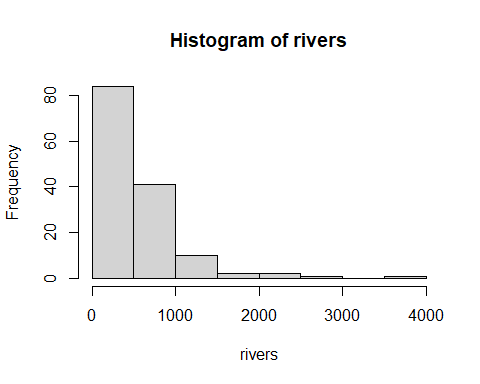
\includegraphics{Homework1_Kyle_Walter_files/figure-latex/unnamed-chunk-2-1.pdf}

The shape of the distribution in plain English is that that more
observations of rivers are seen with length less than 500 and more few
rivers are seen with longer length. The shape of the distribution
appears to be a Poisson. Which makes sense as the number of rivers in
North America is a discrete number, ie one cannot observe half a river,
and the rivers with length were observed a fixed point in time.

\end{document}
